\chapter{均勻空間的幾何}

\lectureoverview{平坦性是對觀測宇宙極佳的近似，但它不是一項原理。若保留均勻性與各向同性，同時允許曲率存在，就會得到三種單連通的空間幾何：歐幾里得空間、球面空間與雙曲空間。這些空間的度規可以根據同心殼層隨距離增長的方式建構；它們的曲率則可透過角大小與天體數量來檢驗。拓撲為環面的平坦空間也可能是有限的。最後，將時間相依的尺度因子乘上上述任一均勻空間的度規，就得到宇宙學的時空度規與哈伯定律；尺度因子的動力學則必須由廣義相對論決定。}

\section{平坦性是觀測結果，不是原理}

到目前為止，我們一直把空間視為平坦，幾乎沒有談到時空幾何。觀測支持把平坦空間當作極佳的近似，但這並不會使平坦性成為定律。測量真正告訴我們的是，任何曲率半徑都必須遠大於我們已經勘測的區域。空間可能恰好平坦，也可能具有正曲率或負曲率。至於遠超可觀測區域的尺度上哪種描述才正確，目前仍不得而知。

因此，我們放寬一項假設，同時保留另一項。我們不再假設空間平坦，但仍假設空間均勻且各向同性。這是工作假設，不是信條。為了了解它的後果，我們先採用這項假設進行計算；之後也可以放棄它，探討非均勻宇宙會有何不同。

均勻性表示每一點的幾何性質都相同。觀測者移到別處，重做局部幾何實驗，會得到相同結果。各向同性則表示沒有任何方向受到偏好。這些條件排除了我們最先想到、幾乎所有彎曲的曲面。拋物面在頂點附近的彎曲程度比遠離頂點處大；長橢球的兩極與腰部也有所不同。表面有凸起的球，或是解析出山脈與山谷的地球表面，雖然彎曲，卻不均勻。宇宙學要問的是更狹義的問題：
\begin{quote}
哪些空間可以是彎曲的，卻仍從每一點、每個方向看來都具有相同的幾何性質？
\end{quote}

暫且不考慮全域識別，可得三種常曲率的答案：平坦空間、正曲率的球面空間，以及負曲率的雙曲空間。全域識別這項限定很重要；稍後我們會建構一個有限的平坦環面，並修正「這三種幾何涵蓋所有可能性」這種過度簡化的說法。

\section{度規與觀測者的座標}

我們先只討論空間，不談時空。空間的幾何由度規描述：度規給出相鄰兩點之間的距離平方\(ds^2\)。只要知道各處的這項局部規則，就能由此求出長度、角度、面積、體積、測地線與曲率。

在歐幾里得平面與三維歐幾里得空間中，笛卡兒座標下的度規為
\begin{equation}
ds_2^2=dx^2+dy^2,
\qquad
ds_3^2=dx^2+dy^2+dz^2.
\label{eq:c03-cartesian-flat}
\end{equation}
加入第三維，只是多出一個正交項\(dz^2\)；但重點不在公式簡單，而在於方程式~\eqref{eq:c03-cartesian-flat}完整指定了局部幾何。

\begin{figure}[htbp]
\centering
\includegraphics[width=0.74\textwidth]{lecture_03_figure_02.png}
\caption{黑板上寫出的平坦三維空間笛卡兒度規。}
\label{fig:c03-cartesian-board}
\lectureframe{00:05:13.138}
\end{figure}

笛卡兒座標不容易呈現天文學家觀察宇宙的方式。我們位於一點，朝不同方向向外觀察，再依角度與距離整理所見。在二維宇宙中，觀測者周圍的所有方向會構成一個圓。因此，極座標不只是優雅的表示法；它也揭示了宇宙學所用的角度幾何。

令\(r\)表示徑向距離，\(\theta\)表示方向。同一個歐幾里得平面現在可寫成度規
\begin{equation}
ds^2 = dr^2 + r^2 d\theta^2.
\label{eq:c03-polar-flat}
\end{equation}
對固定的小角度\(d\theta\)而言，橫向間距為\(r\,d\theta\)。觀測者向外移動時，這個間距線性增長，因此它對度規的平方貢獻為\(r^2d\theta^2\)。

角度項本身就是一維空間的度規。圓是一維球面，記作\(S^1\)；單位圓的度規通常寫成
\begin{equation}
d\Omega_1^2 = d\theta^2,
\qquad\text{so that}\qquad
ds^2 = dr^2 + r^2 d\Omega_1^2.
\label{eq:c03-omega-one}
\end{equation}
黑板上寫的是\(d\Omega^2\)，下標無法辨認；根據口頭定義，所指的物件應為\(d\Omega_1^2\)。

\begin{figure}[htbp]
\centering
\includegraphics[width=0.74\textwidth]{lecture_03_figure_03.png}
\caption{平坦空間的極座標草圖與度規。黑板上寫的是\(d\Omega^2\)；講解指出它是單位圓的度規\(d\Omega_1^2=d\theta^2\)。}
\label{fig:c03-polar-board}
\lectureframe{00:08:37.254}
\end{figure}

\begin{figure}[htbp]
\centering
\begin{tikzpicture}[scale=1.2]
\draw[->] (-1.2,0)--(1.8,0);
\draw[->] (0,-1.2)--(0,1.8);
\draw[thick] (0,0)--(1.3,1.1);
\draw (0.7,0.7) node[above] {$r$};
\draw (0.58,0) arc (0:40:0.58);
\draw (0.8,0.22) node {$\theta$};
\end{tikzpicture}
\caption{以觀測者為中心的極座標圖，重繪自方程式~\eqref{eq:c03-omega-one}所用的座標。}
\label{fig:c03-polar-redraw}
\end{figure}

\begin{classroomqa}
\audiencequestion{\(d\theta^2\)真的表示沿圓周的距離嗎？}
\lecturerresponse{是的。在單位圓上，弧長等於以弧度表示的角度，因此相差\(d\theta\)的鄰近兩點，其內在間距平方為\(d\theta^2\)。圓周長是\(2\pi\)；沿圓周積分一圈\(ds=d\theta\)，恰好得到\(2\pi\)。乘上\(r^2\)，就把單位圓放大成平面中半徑為\(r\)的殼層。\lecturetimestamp{00:09:11--00:09:26}}
\end{classroomqa}

\emph{內在}這個詞很重要。若將單位圓嵌入歐幾里得平面，可以用下式描述：
\begin{equation}
x^2 + y^2 = 1.
\end{equation}
這個方程式描述圓如何置於更大的空間中。對只能測量沿圓周距離的居民來說，這項描述並非必要。我們可以把一條柔韌的光纖彎成不規則的閉合迴圈，而不拉伸它。光纖在平面中的形狀會改變，但其內在周長與度規不變。\(\theta\)的等量增量仍代表沿光纖的等距間隔。因此，幾何必須與嵌入所帶來的偶然形狀區分開來。

\begin{figure}[htbp]
\centering
\includegraphics[width=0.64\textwidth]{lecture_03_figure_04.png}
\caption{黑板比較圓形的單位圓與變形的閉合迴圈。若迴圈只彎曲而未拉伸，兩者便具有相同的內在一維度規。}
\label{fig:c03-intrinsic-board}
\lectureframe{00:10:34.205}
\end{figure}

\begin{figure}[htbp]
\centering
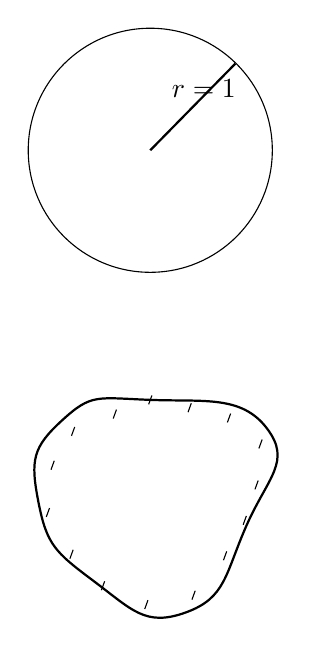
\begin{tikzpicture}[scale=1.0]
\draw (0,0) circle (1.55);
\draw[thick] (0,0)--(1.08,1.1);
\draw (0.68,0.78) node {$r=1$};

\begin{scope}[yshift=-4.35cm]
\draw[thick]
plot[smooth cycle, tension=0.95] coordinates
{(0,1.18) (1.48,0.82) (1.22,-0.42) (0.45,-1.52) (-0.72,-1.12) (-1.42,-0.12) (-1.12,0.92)};
\foreach \p in {(0,1.18),(0.5,1.08),(1.0,0.95),(1.4,0.62),(1.35,0.1),(1.2,-0.35),(0.95,-0.8),(0.55,-1.3),(-0.05,-1.42),(-0.6,-1.18),(-1.0,-0.78),(-1.3,-0.25),(-1.24,0.35),(-0.98,0.78),(-0.45,1.0)}{
\draw[rotate around={70:\p}] \p ++(-0.06,0) -- ++(0.12,0);
}
\end{scope}
\end{tikzpicture}
\caption{外在形變不會改變內在距離：一維空間的居民在兩種嵌入中測得的周長相同。}
\label{fig:c03-intrinsic-redraw}
\end{figure}

現在可以把平坦空間看成以觀測者為中心的一族同心圓。距離\(r\)處的殼層，是放大\(r\)倍的單位圓；這正是因子\(r^2d\Omega_1^2\)所表示的內容。

\section{正曲率：閉合的殼層}

球面是彎曲的，卻是均勻的：在完美球面上，沒有任何一點在幾何上與其他點不同。我們可以不借助外部三維圖像來建構它的度規。想像一群生活在單位\(2\)球面上的二維天文學家，並把他們座標的原點設在自己所在的位置。

距離他們一小段測地距離\(r\)處的圓很小。隨著\(r\)增加，這些圓逐漸變大，在繞球面半圈處達到最大周長，之後縮小，最後在對蹠點收縮成一點。這種增長與收縮是隨\emph{距離}發生，不是隨時間發生。在整個建構過程中，球面都是靜態的。

這裡的\(r\)是沿單位球面的角距離，而非距離某個中心的歐幾里得距離：
\[
0 \le r \le \pi.
\]
在\(r=0\)處是選定的原點，在\(r=\pi/2\)處是繞行半圈的大圓，在\(r=\pi\)處則是對蹠點。此時殼層半徑為\(\sin r\)，因此平坦空間中的因子\(r^2\)改為\(\sin^2r\)：
\begin{equation}
d\Omega_2^2 = dr^2 + \sin^2 r\, d\Omega_1^2
            = dr^2 + \sin^2 r\, d\theta^2.
\label{eq:c03-two-sphere}
\end{equation}
端點與中點的性質恰如所需：
\begin{equation}
\sin 0=0,
\qquad
\sin\frac{\pi}{2}=1,
\qquad
\sin\pi=0.
\end{equation}
因此，殼層從零大小開始，增至最大，最後再次閉合。

\begin{figure}[htbp]
\centering
\includegraphics[width=0.82\textwidth]{lecture_03_figure_05.png}
\caption{從平坦空間的同心圓轉換為球面殼層。畫面中下方的公式部分遭遮擋；口頭推導指出，方程式~\eqref{eq:c03-two-sphere}中的\(r^2\mapsto\sin^2r\)取代了原來的因子。}
\label{fig:c03-spherical-board}
\lectureframe{00:16:11.701}
\end{figure}

\begin{figure}[htbp]
\centering
\resizebox{\linewidth}{!}{%
\begin{tikzpicture}[scale=0.92]
\begin{scope}[xshift=-4.15cm]
\draw[->] (-1.7,0)--(1.9,0);
\draw[->] (0,-1.7)--(0,1.9);
\draw (0,0) circle (0.45);
\draw (0,0) circle (0.9);
\draw (0,0) circle (1.35);
\draw[thick] (0,0)--(1.45,1.2);
\draw (0.56,0.18) arc (18:40:0.63);
\draw (0.94,0.44) node {$\theta$};
\end{scope}

\begin{scope}[xshift=4.15cm]
\draw (0,0) circle (2.0);
\fill (0,-2.0) circle (1.5pt);
\fill (2.0,0) circle (1.5pt);
\fill (0,2.0) circle (1.5pt);
\draw[thick] (0,-2.0) arc (-90:90:2.0);
\draw (0,-2.35) node {$r=0$};
\draw (2.75,0) node {$r=\pi/2$};
\draw (0,2.35) node {$r=\pi$};
\end{scope}
\end{tikzpicture}
}%
\caption{平坦空間的殼層會持續增大；球面殼層則在\(r=\pi/2\)處增至最大，並於\(r=\pi\)處閉合。}
\label{fig:c03-shells-flat-sphere}
\end{figure}

記號\(d\Omega_2^2\)表示單位\(2\)球面的度規，就如同\(d\Omega_1^2\)表示其圓形殼層的度規。同樣的遞迴建構也適用於更高維度。在平坦三維空間中，固定半徑的殼層是\(2\)球面：
\begin{equation}
ds_{\text{flat},3}^2 = dr^2 + r^2 d\Omega_2^2.
\label{eq:c03-flat-three-polar}
\end{equation}
若這些\(2\)球面殼層以因子\(\sin r\)增大後再閉合，所得空間就是單位\(3\)球面：
\begin{equation}
d\Omega_3^2 = dr^2 + \sin^2 r\, d\Omega_2^2.
\label{eq:c03-three-sphere}
\end{equation}
\(3\)球面難以想像，因為要以熟悉的方式嵌入，必須使用四維歐幾里得空間。不過，度規本身已完整描述幾何，不需要圖像。以任一觀測者為中心，都有一層層同心的\(2\)球面；它們先增大到最大，再縮小至對蹠點。

\begin{classroomqa}
\audiencequestion{觀測者位於球面的中心嗎？}
\lecturerresponse{觀測者位於\emph{座標殼層}的中心，卻不位於某個特別的幾何中心。原點只是空間中的一點；任何其他觀測者也能選自己的位置作為\(r=0\)，並得到相同的度規。均勻性正是指沒有任何位置受到偏好。\lecturetimestamp{00:19:21--00:20:27}}
\end{classroomqa}

只為了視覺化，單位圓與單位\(2\)球面可以嵌入歐幾里得空間：
\begin{equation}
x^2+y^2=1,
\qquad
x^2+y^2+z^2=1.
\end{equation}
這些方程式描述的是嵌入，不代表額外的物理。被限制在圓或球面上的螞蟻，可以測出內在度規，無須探測周圍的歐幾里得空間。同樣地，\(S^3\)不是一個帶有神祕邊界的普通球體；它是方程式~\eqref{eq:c03-three-sphere}所描述的完整三維空間。

\section{曲率如何改變我們的觀測}

幾何改變了觀測結果，才成為物理問題。假設某物體的橫向直徑\(d\)已知，其徑向距離\(r\)已透過其他方法推得，並且我們測量了它在天空中的角直徑\(d\theta\)。星系可以提供粗略直觀的例子；更精確的宇宙學則使用經校準的標準尺與標準燭光。距離資訊可以綜合光譜紅移、哈伯關係、光度，以及不同類型天體之間的交叉校準而得。

在平坦空間中，考慮物體橫向寬度上的固定距離\(r\)。由方程式~\eqref{eq:c03-polar-flat}可得
\begin{equation}
d^2 = r^2 d\theta^2.
\label{eq:c03-flat-angle-step}
\end{equation}
因此
\begin{equation}
d\theta = \frac{d}{r}.
\label{eq:c03-flat-angle}
\end{equation}
角大小與距離成反比。

在單位球面上，橫向殼層的大小是\(\sin r\)，而非\(r\)：
\begin{equation}
d^2 = \sin^2 r\, d\theta^2,
\qquad\text{hence}\qquad
d\theta = \frac{d}{\sin r}.
\label{eq:c03-spherical-angle}
\end{equation}
當\(0<r<\pi\)時，\(\sin r<r\)，所以同一物體在相同徑向距離處看起來會比在平坦空間中更大。它的角大小會先減小，在赤道處達到最小，接著隨殼層收縮而增大。在對蹠點處的理想極限下，所有方向都會匯聚，影像則延展至整個天空。

\begin{classroomqa}
\audiencequestion{從宇宙微波背景推論曲率，用的也是這個概念嗎？}
\lecturerresponse{是的。早期電漿的聲學振盪提供了一個特徵物理尺度。我們測量這把標準尺張成的角度，再與各種幾何預測的角度比較。相關天體不必是星系；關鍵是將已知的橫向尺度與觀測到的角大小相比。\lecturetimestamp{00:37:37--00:38:12}}
\end{classroomqa}

殼層體積提供另一種檢驗。在三維平坦空間中，殼層面積正比於\(r^2\)；在單位\(3\)球面上，則正比於\(\sin^2r\)。因此，均勻分布的天體在球面殼層上的數量會先隨距離增加，越過赤道後再減少。相較於平坦空間，正曲率預測出一組成對的訊號：足夠遠的標準尺看起來過大，而足夠遠的殼層包含的天體過少。

\begin{figure}[htbp]
\centering
\resizebox{\linewidth}{!}{%
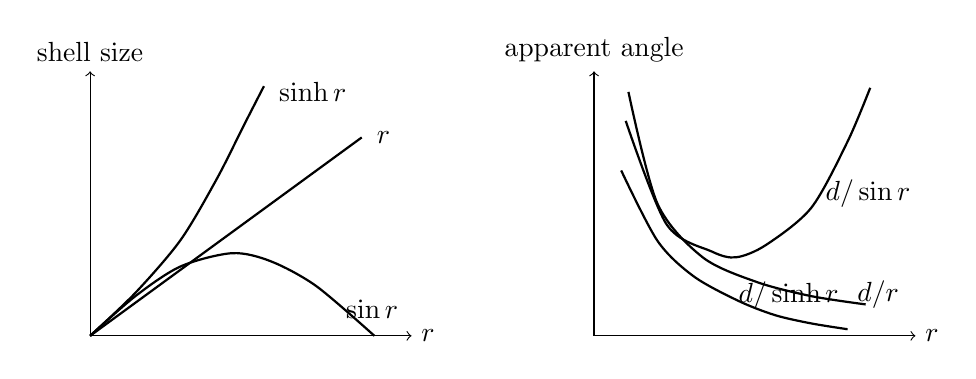
\begin{tikzpicture}[x=1.15cm,y=1.05cm]
\begin{scope}
\draw[->] (0,0)--(3.55,0) node[right] {$r$};
\draw[->] (0,0)--(0,3.2) node[above] {shell size};

\draw[thick] (0,0)--(3.0,2.4);
\draw (3.06,2.4) node[right] {$r$};

\draw[thick]
plot[smooth] coordinates {(0,0) (0.5,0.48) (1.0,0.84) (1.57,1.0) (2.0,0.9) (2.5,0.6) (3.14,0)};
\draw (2.72,0.55) node[below right] {$\sin r$};

\draw[thick]
plot[smooth] coordinates {(0,0) (0.5,0.52) (1.0,1.16) (1.4,1.9) (1.7,2.55) (1.92,3.02)};
\draw (1.98,2.95) node[right] {$\sinh r$};
\end{scope}

\begin{scope}[xshift=6.4cm]
\draw[->] (0,0)--(3.55,0) node[right] {$r$};
\draw[->] (0,0)--(0,3.2) node[above] {apparent angle};

\draw[thick]
plot[smooth] coordinates {(0.38,2.95) (0.7,1.6) (1.2,0.95) (1.8,0.65) (2.4,0.48) (3.0,0.38)};
\draw (2.8,0.5) node[right] {$d/r$};

\draw[thick]
plot[smooth] coordinates {(0.35,2.6) (0.8,1.35) (1.3,1.02) (1.57,0.95) (1.9,1.1) (2.4,1.55) (2.8,2.35) (3.05,3.0)};
\draw (2.45,1.72) node[right] {$d/\sin r$};

\draw[thick]
plot[smooth] coordinates {(0.3,2.0) (0.7,1.15) (1.1,0.72) (1.6,0.42) (2.0,0.25) (2.4,0.15) (2.8,0.08)};
\draw (2.15,0.2) node[above] {$d/\sinh r$};
\end{scope}
\end{tikzpicture}
}%
\caption{徑向殼層因子及相應的角大小定律。正曲率使殼層閉合；負曲率則使殼層呈指數增長。}
\label{fig:c03-shell-angular-laws}
\end{figure}

\begin{classroomqa}
\audiencequestion{沿球面繞行時，徑向座標會變成無窮大嗎？}
\lecturerresponse{不會。在單位球面上，\(r\)表示測地角距離，其範圍僅從\(0\)到\(\pi\)。在\(r=\pi\)處，殼層已在對蹠點收縮成一點。這裡探討的是固定的空間幾何，不是追蹤物體隨時間向外運動。稍後引入曲率半徑時，所有物理距離都會乘上該半徑，但這個無量綱座標的範圍不變。\lecturetimestamp{00:39:30--00:40:35}}
\end{classroomqa}

\section{投影不是幾何}

在轉向負曲率之前，不妨先看看圖像能如何嚴重扭曲原本忠實的幾何。將球面放在與南極相切的平面上。從北極經過球面上的每一點\(P\)畫一條直線，並延伸至平面上的\(P'\)。這就是球極投影。北極本身會投影至無窮遠。南極附近的小區域在平面上的表示幾乎沒有失真；北極附近面積相同的內在區域，投影到平面後卻變得極其巨大。

失真來自地圖，不是球面。球面本身仍然均勻，儘管它的平面影像為幾何上等價的區域賦予了極不相同的座標大小。稍後把無限的雙曲空間壓縮到有限圓盤時，也需要記住這一點。

\begin{figure}[htbp]
\centering
\resizebox{\linewidth}{!}{%
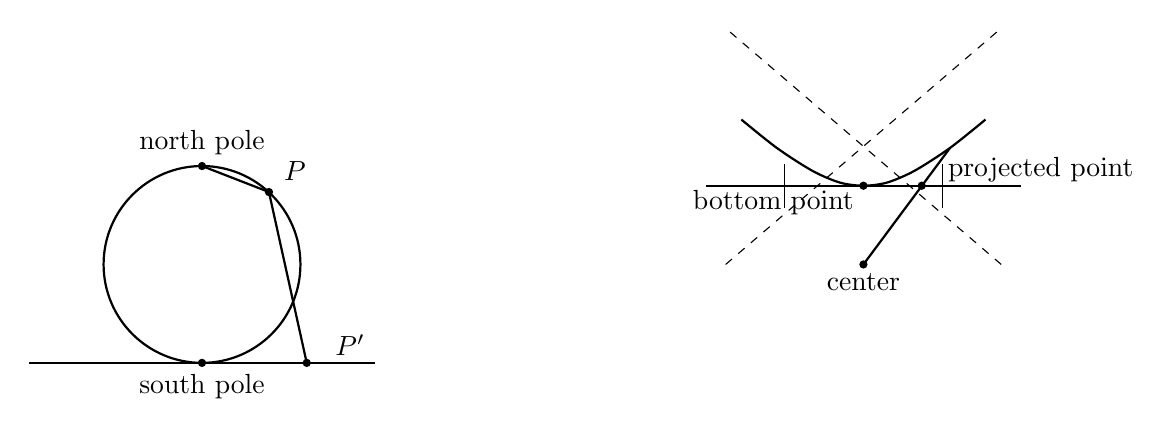
\begin{tikzpicture}[scale=1.0]
\begin{scope}[xshift=-4.2cm]
\draw[thick] (-2.2,-1.25)--(2.2,-1.25);
\draw[thick] (0,0) circle (1.25);
\fill (0,1.25) circle (1.5pt);
\fill (0,-1.25) circle (1.5pt);
\draw (0,1.55) node {north pole};
\draw (0,-1.55) node {south pole};

\fill (0.85,0.92) circle (1.5pt);
\draw (0.92,1.18) node[right] {$P$};
\draw[thick] (0,1.25)--(0.85,0.92)--(1.33,-1.25);
\fill (1.33,-1.25) circle (1.5pt);
\draw (1.57,-1.03) node[right] {$P'$};
\end{scope}

\begin{scope}[xshift=4.2cm]
\draw[thick] (-2.0,1)--(2.0,1);
\draw[dashed] (-1.75,0)--(1.75,3.0);
\draw[dashed] (1.75,0)--(-1.75,3.0);
\draw[thick]
plot[smooth] coordinates
{(-1.55,1.84) (-1.1,1.48) (-0.65,1.19) (-0.3,1.04) (0,1.0) (0.3,1.04) (0.65,1.19) (1.1,1.48) (1.55,1.84)};
\fill (0,0) circle (1.5pt);
\fill (0,1) circle (1.5pt);
\draw (0,-0.22) node {center};
\draw (0,0.78) node[left] {bottom point};
\draw[thick] (0,0)--(1.1,1.48);
\fill (0.74,1.0) circle (1.5pt);
\draw (0.95,1.2) node[right] {projected point};
\draw (-1,0.72) -- (-1,1.28);
\draw (1,0.72) -- (1,1.28);
\end{scope}
\end{tikzpicture}
}%
\caption{左圖：球極投影將球面的北極投影至無窮遠。右圖：雙曲面可投影至有限圓盤，此處以截面的一段表示。座標失真不會破壞內在均勻性。}
\label{fig:c03-projections}
\end{figure}

\section{負曲率：殼層比平坦空間增長得更快}

第三種單連通的均勻幾何，以雙曲正弦取代\(\sin r\)。二維與三維單位空間的度規為
\begin{equation}
dh_2^2 = dr^2 + \sinh^2 r\, d\Omega_1^2,
\label{eq:c03-hyperbolic-two}
\end{equation}
\begin{equation}
dh_3^2 = dr^2 + \sinh^2 r\, d\Omega_2^2.
\label{eq:c03-hyperbolic-three}
\end{equation}
座標\(r\)的範圍則是
\begin{equation}
0\le r<\infty.
\end{equation}
在原點附近，\(\sinh r\approx r\)，因此幾何在局部近似歐幾里得。遠處的殼層比歐幾里得空間中的殼層增長快得多，而且不會折返。

增長關係可由下式看出：
\begin{equation}
\sin r = \frac{e^{ir}-e^{-ir}}{2i},
\qquad
\sinh r = \frac{e^r-e^{-r}}{2}.
\label{eq:c03-sin-sinh}
\end{equation}
當\(r\)很大時，\(\sinh r\sim e^r/2\)。因此在二維中，圓周長隨半徑呈指數增長；在三維中，殼層面積則按\(\sinh^2r\sim e^{2r}/4\)增長。均勻分布的天體在遙遠殼層上的數量也相應更多。

對橫向大小為\(d\)的物體，
\begin{equation}
d^2 = \sinh^2 r\, d\theta^2,
\qquad\text{so}\qquad
d\theta = \frac{d}{\sinh r}.
\label{eq:c03-hyperbolic-angle}
\end{equation}
當\(r\)很大時，
\begin{equation}
d\theta \sim 2d\,e^{-r}.
\end{equation}
因此，負曲率呈現與正曲率相反的特徵：遙遠的標準尺看起來過小，而遙遠殼層中的天體數量則多於平坦空間的預測。

\begin{classroomqa}
\audiencequestion{球面與雙曲空間的徑向範圍有何不同？}
\lecturerresponse{在單位球面上，\(r\)到達對蹠點時便停止，也就是\(r=\pi\)。在雙曲空間中，座標則沒有上限，\(0\le r<\infty\)。殼層因子也顯示出同樣的差別：\(\sin r\)會回到零，\(\sinh r\)則持續增大。\lecturetimestamp{00:52:46--00:53:25}}
\end{classroomqa}

有一種嵌入方式可以幫助理解均勻性。引入環境座標\(T,x,y\)，其中\(T\)只是嵌入座標，\emph{不是}宇宙學時間；接著取上半葉
\begin{equation}
T^2 - x^2 - y^2 = 1.
\label{eq:c03-hyperboloid}
\end{equation}
並在環境空間中採用洛侖茲號差度規
\begin{equation}
d\ell_{\mathrm{emb}}^2=-dT^2+dx^2+dy^2.
\label{eq:c03-ambient-minkowski}
\end{equation}
雙曲面上誘導出的度規是正定的。洛侖茲變換會同時保持方程式~\eqref{eq:c03-hyperboloid}與~\eqref{eq:c03-ambient-minkowski}\allowbreak，並且能將上半葉上的任一點變換至任意另一點。就此而言，在雙曲空間中更換原點，類似於在輔助的環境空間中傾斜時間軸。所有點在幾何上都等價。

將雙曲面投影至圓盤後，無窮遠處的點會聚集在邊界圓上。鄰近區域的圖像幾乎不失真；越遠的區域則受到越強烈的壓縮。這就是天使與魔鬼重複圖案中常見的Poincar\'e圓盤模型。座標變換可以將邊緣附近看來很小的圖形移至中心，使它在那裡變大，同時維持所有內在長度與角度。在三維中，相應的模型是球體而不是圓盤。\emph{Poincar\'e空間}、\emph{羅巴切夫斯基空間}與\emph{均勻負曲率空間}都是指同一種局部幾何。

\begin{classroomqa}
\audiencequestion{有限圓盤和彭羅斯圖類似嗎？}
\lecturerresponse{兩者相似之處僅在於都把無限區域表示在有限圖像內。不過，這裡的圓盤表示的是空間，不是時空或因果無窮。圖上的圓盤邊界雖位於有限的座標半徑，在內在的雙曲度規中卻遠在無窮處。\lecturetimestamp{01:02:55--01:03:05}}
\end{classroomqa}

\section{曲率半徑}

目前寫出的度規描述的是單位幾何。若要讓球面或雙曲空間具有任意曲率半徑，就將所有長度乘上一個常數。黑板上以\(a\)表示這個常數；為避免與稍後使用的時間相依宇宙學尺度因子混淆，我們把靜態曲率半徑記作\(R_c\)。由於度規量度的是長度平方，
\begin{align}
ds_{\mathrm{sph}}^2
  &=R_c^2d\Omega_n^2
   =R_c^2\left(dr^2+\sin^2r\,d\Omega_{n-1}^2\right),\\
ds_{\mathrm{hyp}}^2
  &=R_c^2dh_n^2
   =R_c^2\left(dr^2+\sinh^2r\,d\Omega_{n-1}^2\right).
\label{eq:c03-scaled-curvature}
\end{align}
物理徑向距離為\(R_cr\)。增大\(R_c\)會使空間的曲率減小；常截面曲率的絕對值按\(1/R_c^2\)縮放。當\(R_c\to\infty\)時，兩種彎曲度規在任何固定的有限區域內都會趨近歐幾里得幾何。

\begin{classroomqa}
\audiencequestion{如果把球面放大為兩倍，它會變得更彎曲，還是更不彎曲？}
\lecturerresponse{更不彎曲。課堂上最初的回答，後來透過比較籃球與地球而得到修正：較小的表面在相同距離內彎得更急。將\(R_c\)加倍，會使反曲率半徑的尺度減半，並使截面曲率\(1/R_c^2\)縮小為四分之一。\lecturetimestamp{01:10:14--01:10:56}}
\end{classroomqa}

這說明了為什麼三種幾何在近處看起來相同。當\(r\ll1\)時，
\begin{equation}
\sin r=r-\frac{r^3}{6}+\cdots,
\qquad
\sinh r=r+\frac{r^3}{6}+\cdots.
\end{equation}
兩種彎曲度規的首項都是平坦空間的極座標度規；曲率最早出現在相對量級為\((L/R_c)^2\)、對應物理尺度\(L\)的修正項中。

\begin{classroomqa}
\audiencequestion{觀測能判定空間是平坦、球面或雙曲的嗎？}
\lecturerresponse{觀測告訴我們，可觀測區域非常接近平坦。課堂上的粗略估計是：曲率效應若受到百分之一的限制，便表示\(R_c\)至少約為可見區域尺度的十倍，因為\((L/R_c)^2\lesssim10^{-2}\)。相應的曲率體積至少約為\(10^3\)個可見宇宙體積。這是課堂上的數量級估計，不是引用當前精密資料所得的數值；空間恰好平坦仍是\(R_c=\infty\)這種可能性。\lecturetimestamp{01:11:00--01:13:37}}
\end{classroomqa}

\section{平坦但有限：環面}

現在必須修正「平坦、球面與雙曲空間是僅有的均勻空間」這種說法。它們是三種單連通的常曲率幾何。平坦空間也可能具有非平凡的全域拓撲。

先從歐幾里得矩形開始。將左邊的每一點與右邊對應的點識別，再將下邊與上邊識別。越過任何一條邊，都會從對邊接回來。局部度規仍是\(dx^2+dy^2\)，但全域空間變成週期性的有限空間。這個商空間是平坦的二維環面\(T^2\)。一個週期維度形成圓\(T^1\)；將長方體的相對面識別，則形成平坦的三維環面\(T^3\)。這種建構可以推廣至任意維度。

\begin{figure}[htbp]
\centering
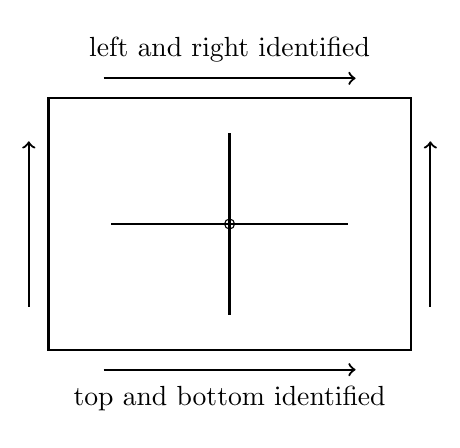
\begin{tikzpicture}[scale=1.0]
\draw[thick] (0,0) rectangle (4.6,3.2);

\draw[->,thick] (0.7,3.45)--(3.9,3.45);
\draw[->,thick] (0.7,-0.25)--(3.9,-0.25);

\draw[->,thick] (-0.25,0.55)--(-0.25,2.65);
\draw[->,thick] (4.85,0.55)--(4.85,2.65);

\draw[thick] (0.8,1.6)--(3.8,1.6);
\draw[thick] (2.3,0.45)--(2.3,2.75);

\draw (2.3,1.6) circle (1.8pt);

\draw (2.3,-0.62) node {top and bottom identified};
\draw (2.3,3.82) node {left and right identified};
\end{tikzpicture}
\caption{將矩形的相對邊識別後，即構成平坦環面。邊緣不是邊界；每對對應的點在商空間中是同一點。}
\label{fig:c03-flat-torus}
\end{figure}

\begin{classroomqa}
\audiencequestion{所以，宇宙可以既平坦又有限嗎？}
\lecturerresponse{可以。平坦性是關於度規的局部陳述；有限性則可能是關於拓撲的全域陳述。若三維環面夠大，在我們能觀測到的整個區域內，它看起來都會是歐幾里得空間，儘管總體積有限。\lecturetimestamp{01:13:37--01:17:59}}
\end{classroomqa}

萬有覆疊圖像能清楚呈現可觀測的後果。不要識別矩形的邊，而是用基本矩形的副本鋪滿無限的歐幾里得平面。環面上的同一個物體會在每個副本中各出現一次。在三維中，這些副本會形成類似週期晶體的排列。

\begin{classroomqa}
\audiencequestion{我們能住在環面宇宙中而毫無察覺嗎？}
\lecturerresponse{可以，只要基本胞元比光已經傳到我們所在區域的範圍還大。如果胞元夠小，光就能穿過識別邊界；我們可能會在不同方向看到同一批星系的重複影像，甚至看到自己周遭區域的重複影像。無論是哪種情況，局部幾何仍然平坦。\lecturetimestamp{01:18:16--01:22:04}}
\end{classroomqa}

\begin{classroomqa}
\audiencequestion{為什麼球面會在對蹠點停止，而環面卻會重複？}
\lecturerresponse{在球面上，周圍的殼層確實會在\(r=\pi\)處收縮至零；所有徑向方向都在對蹠點會合。在環面上，所選矩形胞元的邊緣不會收縮。它與同樣大的對邊識別，因此越過邊緣，只是在週期座標的描述中繼續穿越同一空間。\lecturetimestamp{01:22:06--01:23:02}}
\end{classroomqa}

\section{從空間到時空}

現在可以把時間加回來。在光速取\(c=1\)的單位制中，閔考斯基度規為
\begin{equation}
ds^2 = -dt^2 + dx^2 + dy^2 + dz^2.
\label{eq:c03-minkowski}
\end{equation}
符號慣例可以自行選擇；重要的是時間項的符號與空間項相反。光線沿零軌跡傳播：
\begin{equation}
ds^2 = 0.
\end{equation}
若只沿\(x\)方向運動，則
\begin{equation}
-dt^2 + dx^2 = 0
\qquad\Rightarrow\qquad
dx = \pm dt.
\label{eq:c03-null-flat}
\end{equation}
正負號分別表示光以單位速率向左或向右傳播。

在宇宙學中，保留固有時項\(-dt^2\)，將歐幾里得空間部分換成均勻空間的度規，並讓其整體尺度隨時間變化。我們以\(a(t)\)表示這個尺度因子。它現在是動力學函數，而非靜態比較中所用的固定半徑\(R_c\)。

以可視化的\(2+1\)維空間為例，考慮
\begin{equation}
ds^2 = -dt^2 + a(t)^2 d\Omega_2^2.
\label{eq:c03-two-plus-one}
\end{equation}
在每個固定的\(t\)時刻，空間都是半徑為\(a(t)\)的\(2\)維球面。將這些球面沿時間堆疊，就構成時空。熟悉的\(3+1\)維建構為
\begin{equation}
ds^2 = -dt^2 + a(t)^2 d\Sigma^2,
\label{eq:c03-frw-general}
\end{equation}
其中\(d\Sigma^2\)是與時間無關的單位空間度規。三種單連通情形為
\begin{align}
\text{flat:}\quad
ds^2&=-dt^2+a(t)^2\left(dx^2+dy^2+dz^2\right),\label{eq:c03-frw-flat}\\
\text{spherical:}\quad
ds^2&=-dt^2+a(t)^2d\Omega_3^2,\label{eq:c03-frw-spherical}\\
\text{hyperbolic:}\quad
ds^2&=-dt^2+a(t)^2dh_3^2.\label{eq:c03-frw-hyperbolic}
\end{align}
共動座標之間的相對尺度固定，而\(a(t)\)隨時間變化。在球面與雙曲空間的正規化中，\(a(t)\)也就是瞬時曲率半徑。在平坦情形中，其絕對尺度可吸收到共動座標裡。

無須先施加任何引力場方程式，就能推出哈伯定律。考慮兩個相鄰的共動點，令它們的座標間距\(\chi\)固定。兩點之間的物理距離為
\begin{equation}
D(t)=a(t)\chi.
\label{eq:c03-comoving-distance}
\end{equation}
在固定\(\chi\)下微分，可得
\begin{equation}
V=\dot D=\dot a(t)\chi.
\end{equation}
消去\(\chi\)，得到
\begin{equation}
V = \frac{\dot a}{a} D.
\label{eq:c03-hubble-law}
\end{equation}
因此
\begin{equation}
H = \frac{\dot a}{a}.
\label{eq:c03-hubble-parameter}
\end{equation}
這是均勻膨脹或收縮的運動學恆等式，適用於三種空間幾何：當\(\dot a>0\)時，兩點彼此遠離；當\(\dot a<0\)時，兩點彼此接近。

僅憑幾何無法確定\(a(t)\)。例如\begin{equation}
a(t)\propto t^{2/3},
\qquad
a(t)\propto t^{1/2},
\qquad
a(t)\propto e^{Ht}
\end{equation}這些函數都符合均勻度規的形式假設，卻描述不同的宇宙物質與能量成分。廣義相對論提供了動力學方程，據此可在這些情形中作出選擇。由此得到的弗里德曼方程，也會把平坦、球面與雙曲情形，分別連結到前面建立的牛頓宇宙學中的零能、負能與正能情形。

\begin{classroomqa}
\audiencequestion{幾何與宇宙的演化，會不會比這些模型複雜得多？}
\lecturerresponse{當然會。均勻性與各向同性是相當嚴格的假設；之所以採用它們，是因為它們符合直觀、在大尺度觀測上相當成功，而且在數學上易於處理。還有許多更複雜的幾何與演化形式。一個重要的動力學問題是：廣泛的一類初始不規則模型，是否會演化成這些簡單的均勻形式之一。\lecturetimestamp{01:36:00--01:36:50}}
\end{classroomqa}

\begin{classroomqa}
\audiencequestion{\(3\)維球面是四維物體的邊界嗎？}
\lecturerresponse{透過嵌入方式可以把它表示成那樣，但宇宙學空間本身就是\(3\)維球面。它有三個內在維度，而且沒有邊界。四維歐幾里得空間中的圖像只是輔助理解的架構；~\eqref{eq:c03-three-sphere}已足以完整定義這個幾何。\lecturetimestamp{01:36:55--01:37:59}}
\end{classroomqa}

\begin{classroomqa}
\audiencequestion{要取得曲率檢驗所需的距離，是否只有光度這一種方法？}
\lecturerresponse{不是。譜線可用來辨識紅移，鄰近的距離階梯可用來校準哈伯關係，而超新星則提供近似標準的光度。這些方法會彼此交叉檢驗，不會只依賴其中一種。即使平方反比光度定律也取決於幾何，因為光前沿的面積由\(r^2\)、\(\sin^2r\)或\(\sinh^2r\)決定。多種觀測量彼此吻合，才支持宇宙近乎平坦的結論。\lecturetimestamp{01:38:00--01:41:07}}
\end{classroomqa}

\section{本節重點}

均勻宇宙的幾何，可以從以任一觀測者為中心的球殼如何增長看出：
\begin{equation}
f(r)=
\begin{cases}
r, & \text{flat space},\\
\sin r, & \text{positive curvature},\\
\sinh r, & \text{negative curvature}.
\end{cases}
\end{equation}
空間度規為\(dr^2+f(r)^2d\Omega_{n-1}^2\)。同一個函數同時決定角尺度與球殼上可觀測到的天體數量，因此曲率具有直接的觀測意義。曲率半徑很大時，這些差異在局部不易顯現；而環面識別則表明，單憑局部曲率無法決定整體大小或拓樸。

在三種均勻空間度規中的任一種加入\(-dt^2\)，並將空間度規乘上共同因子\(a(t)^2\)，即可得到宇宙學時空。如此便可得\(V=HD\)，其中\(H=\dot a/a\)，但\(a(t)\)仍未確定。因此，下一步不再是幾何推演，而是探討動力學：運用愛因斯坦方程，確定物質、輻射、曲率及其他形式的能量如何影響尺度因子的演化。
